\begin{frame}
  \begin{itemize}
    \item Find a way to measure how well a parametric model predicts known
      data (the training set).
    \item Use that information to adjust the
      parameters and make the model more accurate
    \item Repeat until a "good enough" model is found
  \end{itemize}
\end{frame}

\begin{frame}
  \frametitle{The error function}
  \begin{center}
    \begin{equation*}
      \begin{split}
        e(w) & =
        \left \{
          \begin{array}{cl}
            1 & $if $ h_w(x) \neq y \\
            0 & $if $ h_w(x) = y
          \end{array}
          \right.\\~\\
          & = |h_w(x) - y| \\~\\
        \end{split}
      \end{equation*}
    \end{center}
  \end{frame}

  \begin{frame}
    \begin{center}
      $E(w) = \displaystyle\sum_{i = 1}^n{|h_w(x^{(i)}) - y^{(i)}|}$ \\~\\
      "Add 1 for every labeled data where the model is wrong"
    \end{center}
  \end{frame}

  \begin{frame}
    \frametitle{Error function}
    \begin{center}
      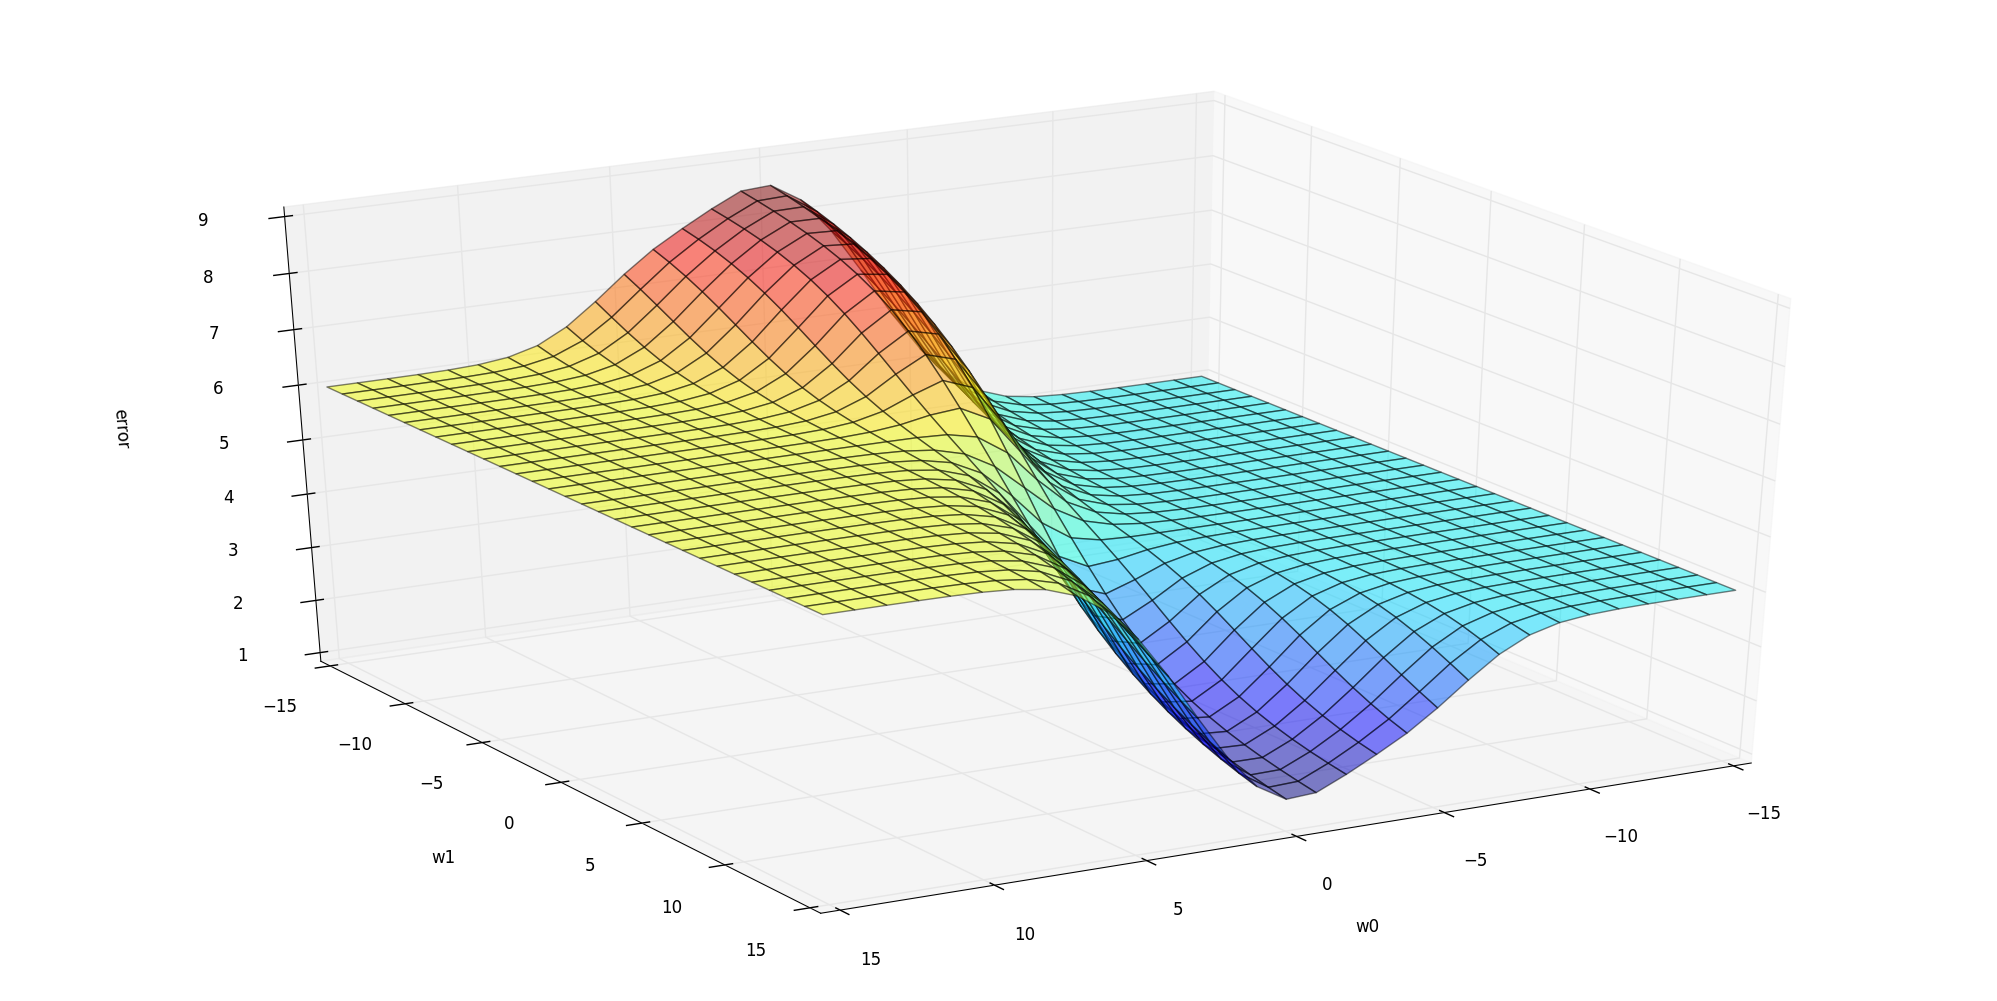
\includegraphics[scale=0.22]{./pictures/error_abs.png}
    \end{center}
  \end{frame}

  \begin{frame}
    \frametitle{The error function}
    \begin{center}
      \begin{equation*}
        \begin{split}
          e(w) & =
          \left \{
            \begin{array}{cl}
              -\log(h_w(x)) & $ if $ y = 1\\
              -\log(1 - h_w(x)) & $ if $ y = 0
            \end{array}
            \right.\\~\\
            & = -y \log(h_w(x)) - (1 - y) \log(1 - h_w(x))\\~\\
          \end{split}
        \end{equation*}
      \end{center}
    \end{frame}

    \begin{frame}
      \frametitle{The logistic function}
      \begin{center}
        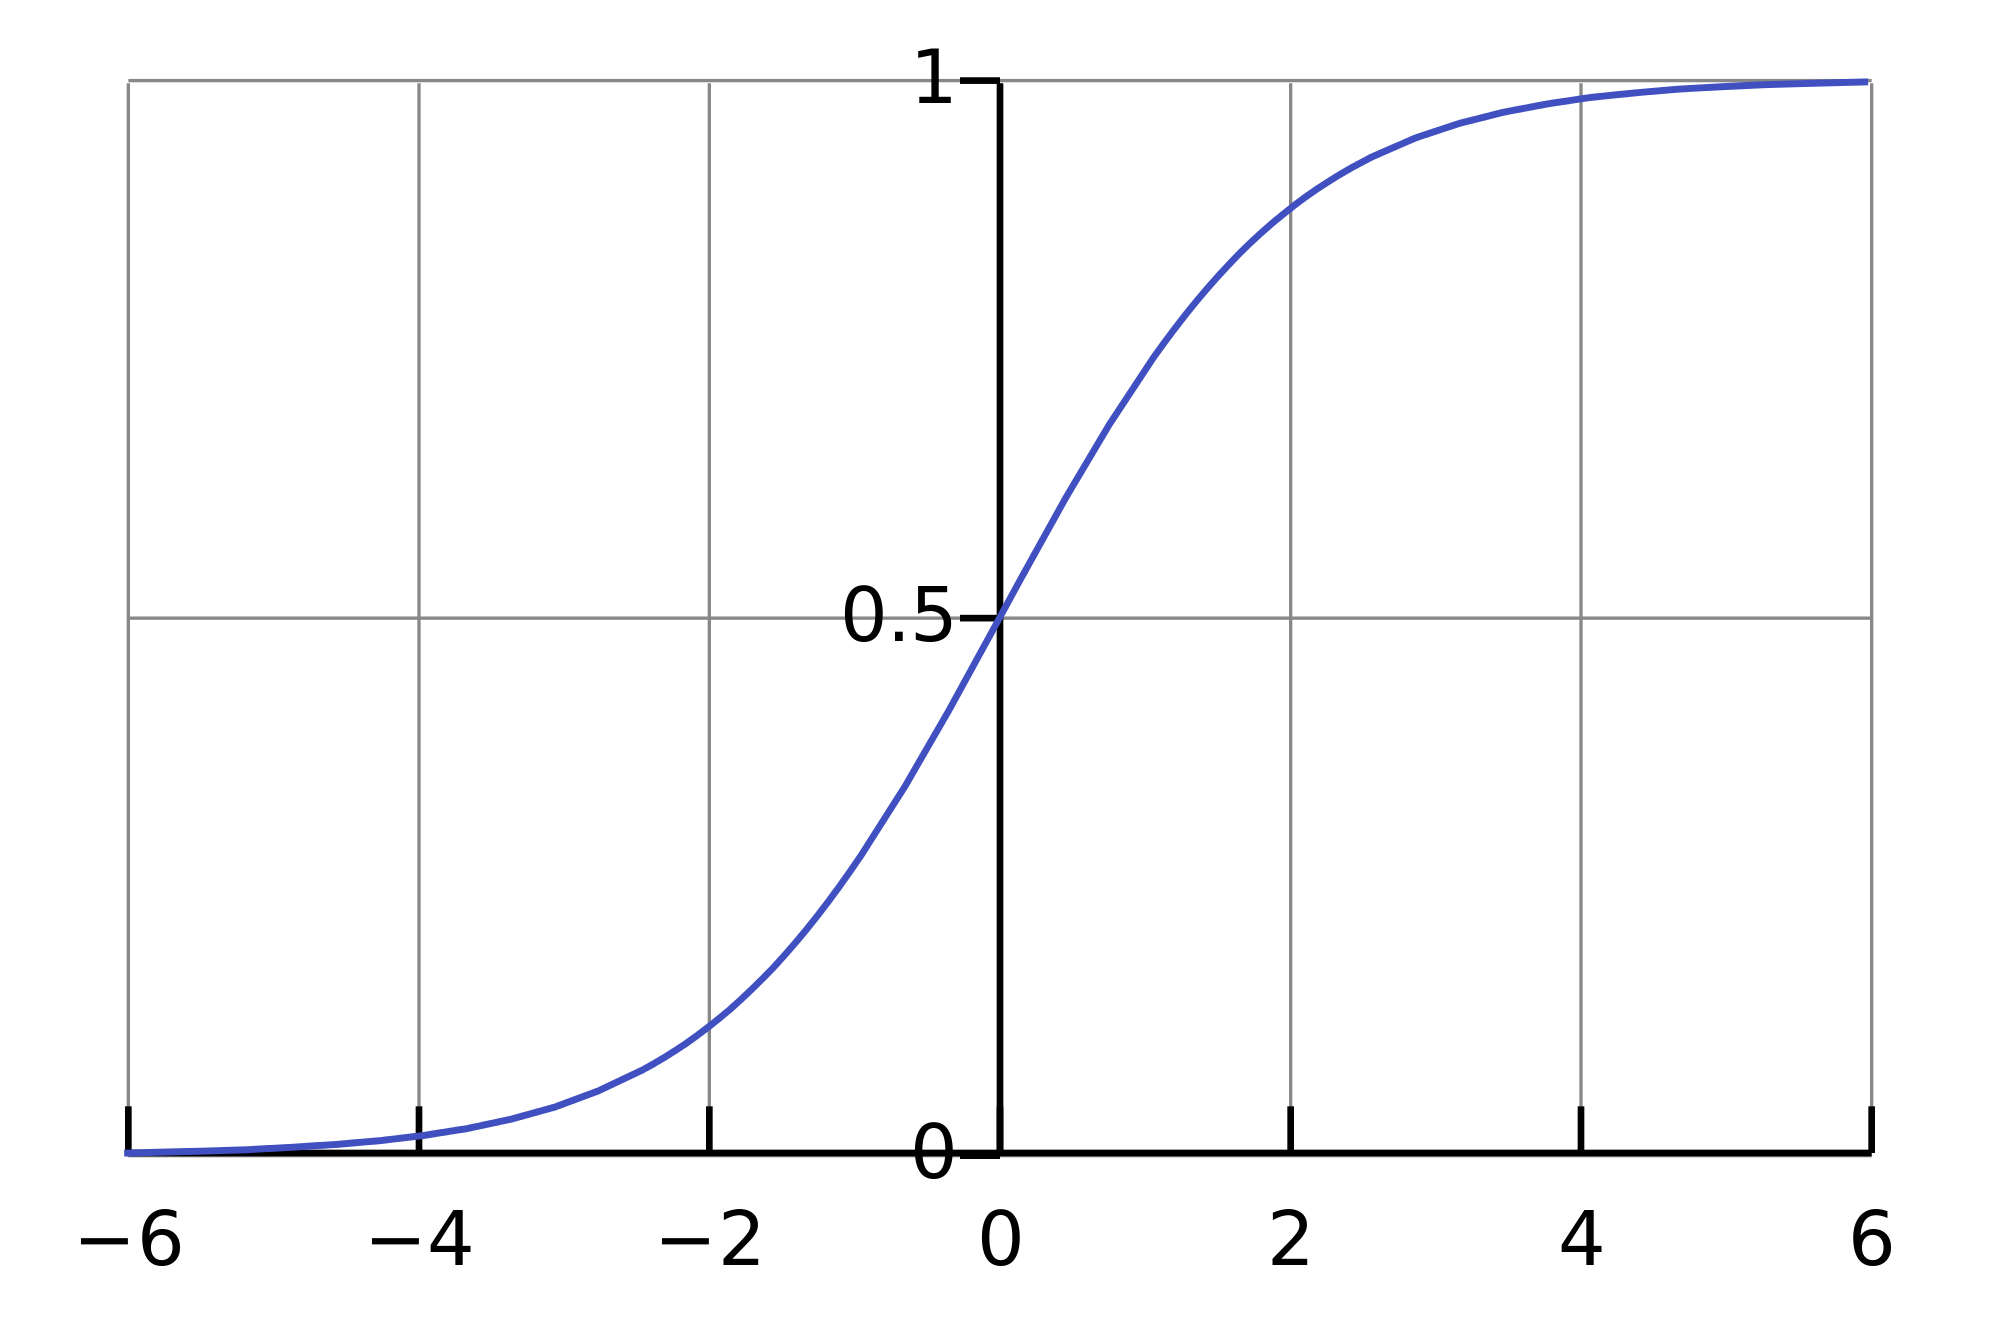
\includegraphics[scale=0.14]{./pictures/sigmoid.png}
      \end{center}
    \end{frame}

    \begin{frame}
      \frametitle{Error function}
      \begin{center}
        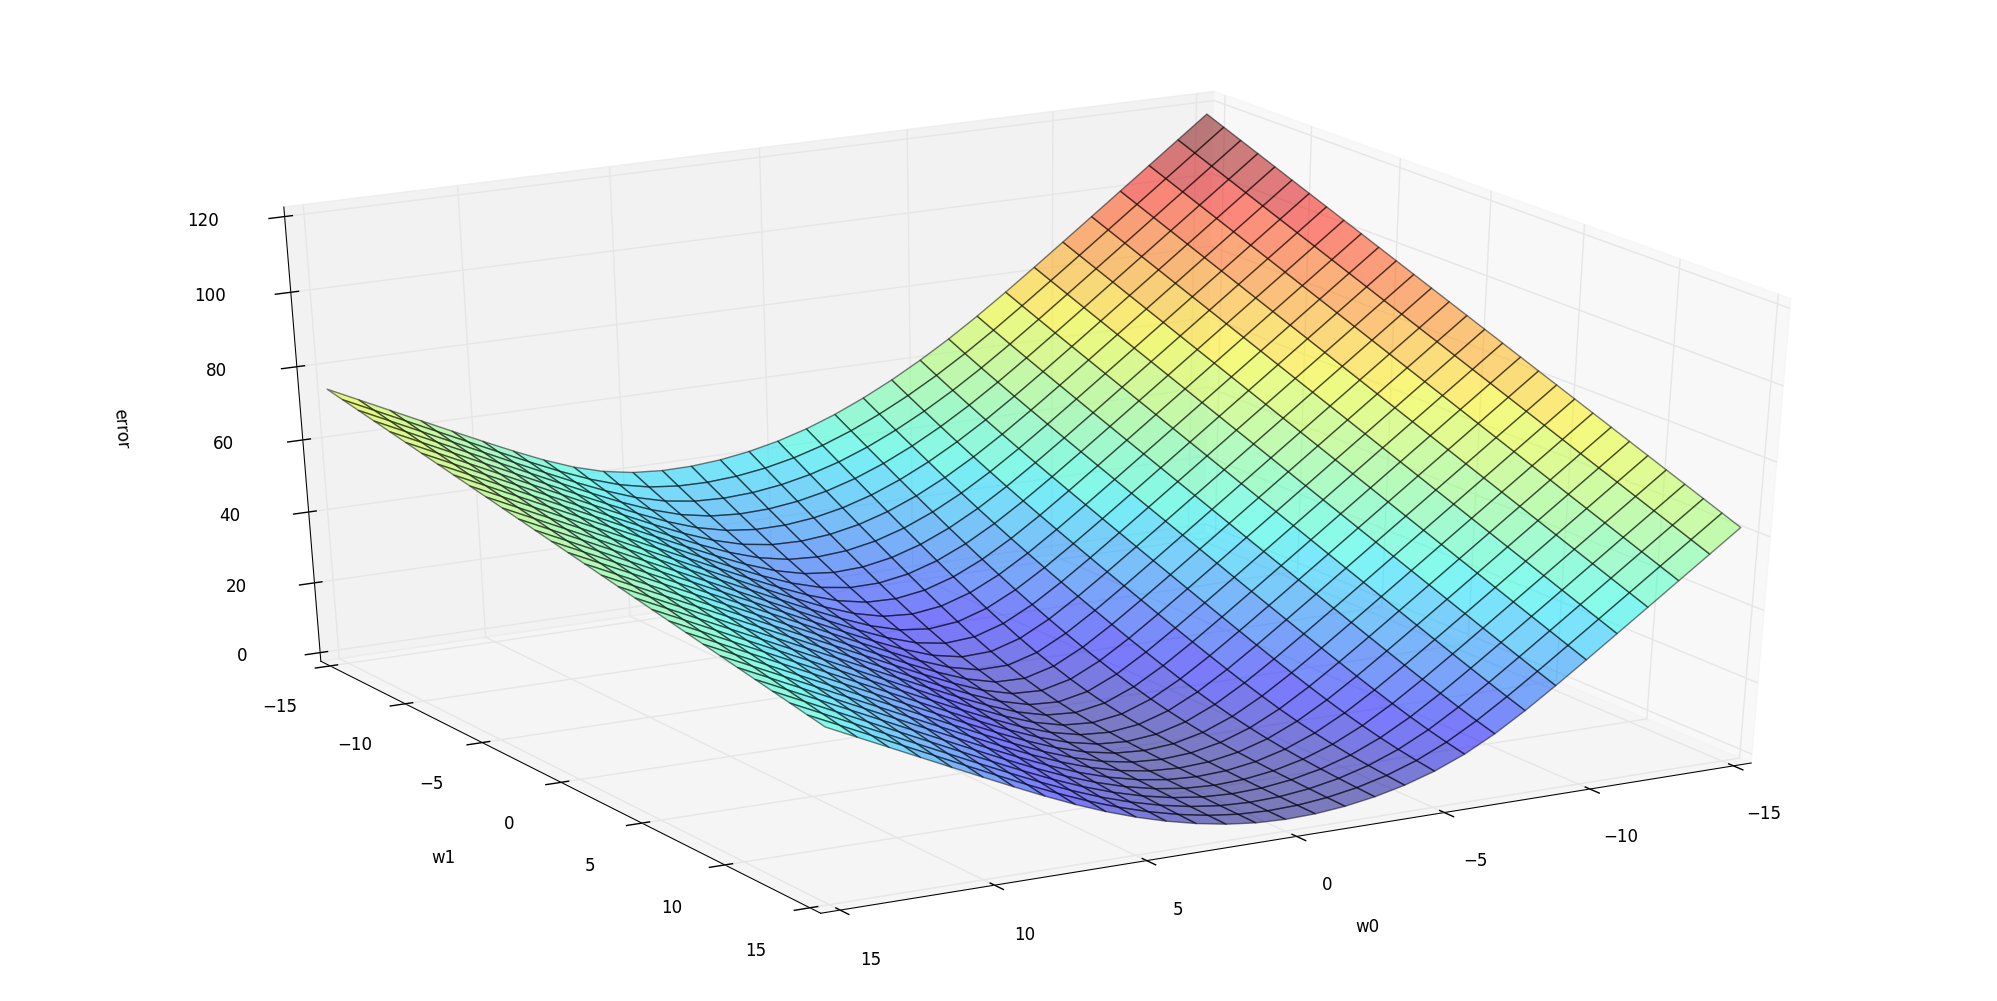
\includegraphics[scale=0.22]{./pictures/error_function.png}
      \end{center}
    \end{frame}

    \begin{frame}
      \begin{equation*}
        \begin{split}
          \frac{\partial e}{\partial w} & = \frac{\partial \displaystyle\sum_{i =
        1}^n{-y \log(h_w(x)) - (1 - y) \log(1 -
      h_w(x)})}{\partial w} \\~\\
      & = \displaystyle\sum_{i = 1}^n{\frac{\partial(-y \log(g(x \cdot
  w)) - (1 - y) \log(1 - g(x \cdot w)))}{\partial w}} \\
\end{split}
  \end{equation*}
\end{frame}

\begin{frame}
  \begin{equation*}
    E(w)
  \end{equation*}
\end{frame}

\begin{frame}[fragile]
  \begin{block}{Logistic function}
    \begin{lstlisting}
      def g(x):
      1 / (1 + exp(-x))
    \end{lstlisting}
  \end{block}
\end{frame}

\begin{frame}
  \frametitle{Gradient descent}
  \begin{center}
    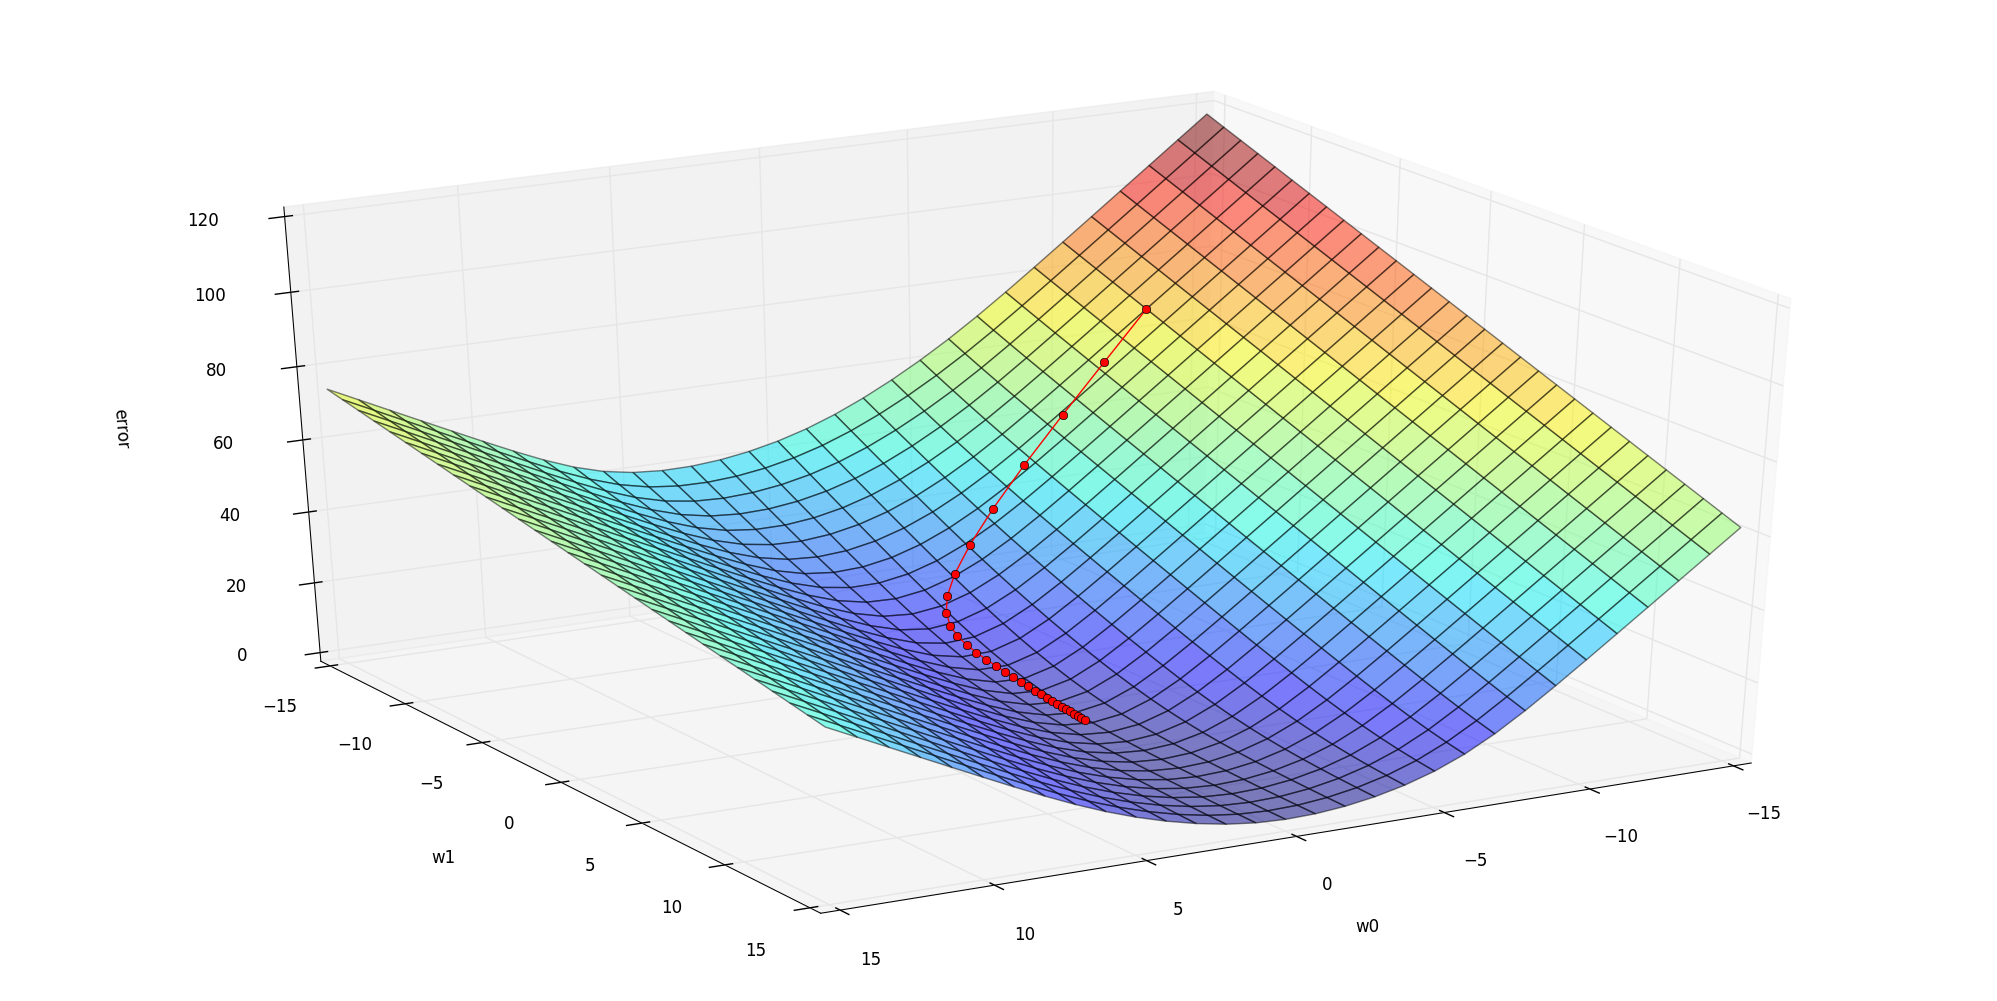
\includegraphics[scale=0.22]{./pictures/gradient_descent.png}
  \end{center}
\end{frame}

\begin{frame}
  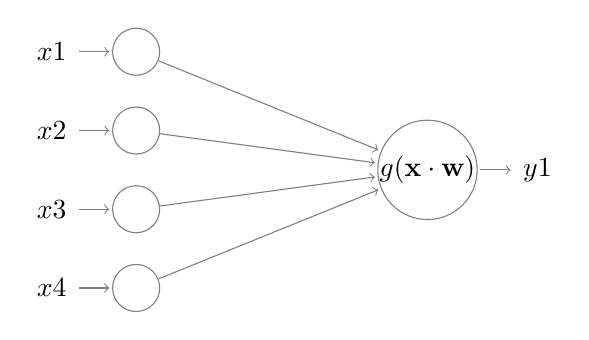
\begin{tikzpicture}[shorten >=1pt,->,draw=black!50, node distance=2.5cm]
    \tikzstyle{every pin edge}=[<-,shorten <=1pt]
    \tikzstyle{neuron}=[circle,draw,minimum size=17pt,inner sep=0pt]

    \foreach \y in {1,2,3,4}
    \node[neuron, pin=left:$x\y$] (I-\y) at (0,-\y) {};

    \node[neuron,pin={[pin edge={->}]right:$y1$}, right of=I-3] (O-1) at
    (1.2,-2.5) {$g(\textbf{x} \cdot \textbf{w})$};

    \foreach \src in {1,2,3,4}
    \path (I-\src) edge (O-1);
  \end{tikzpicture}
\end{frame}

\begin{frame}
  \begin{center}
    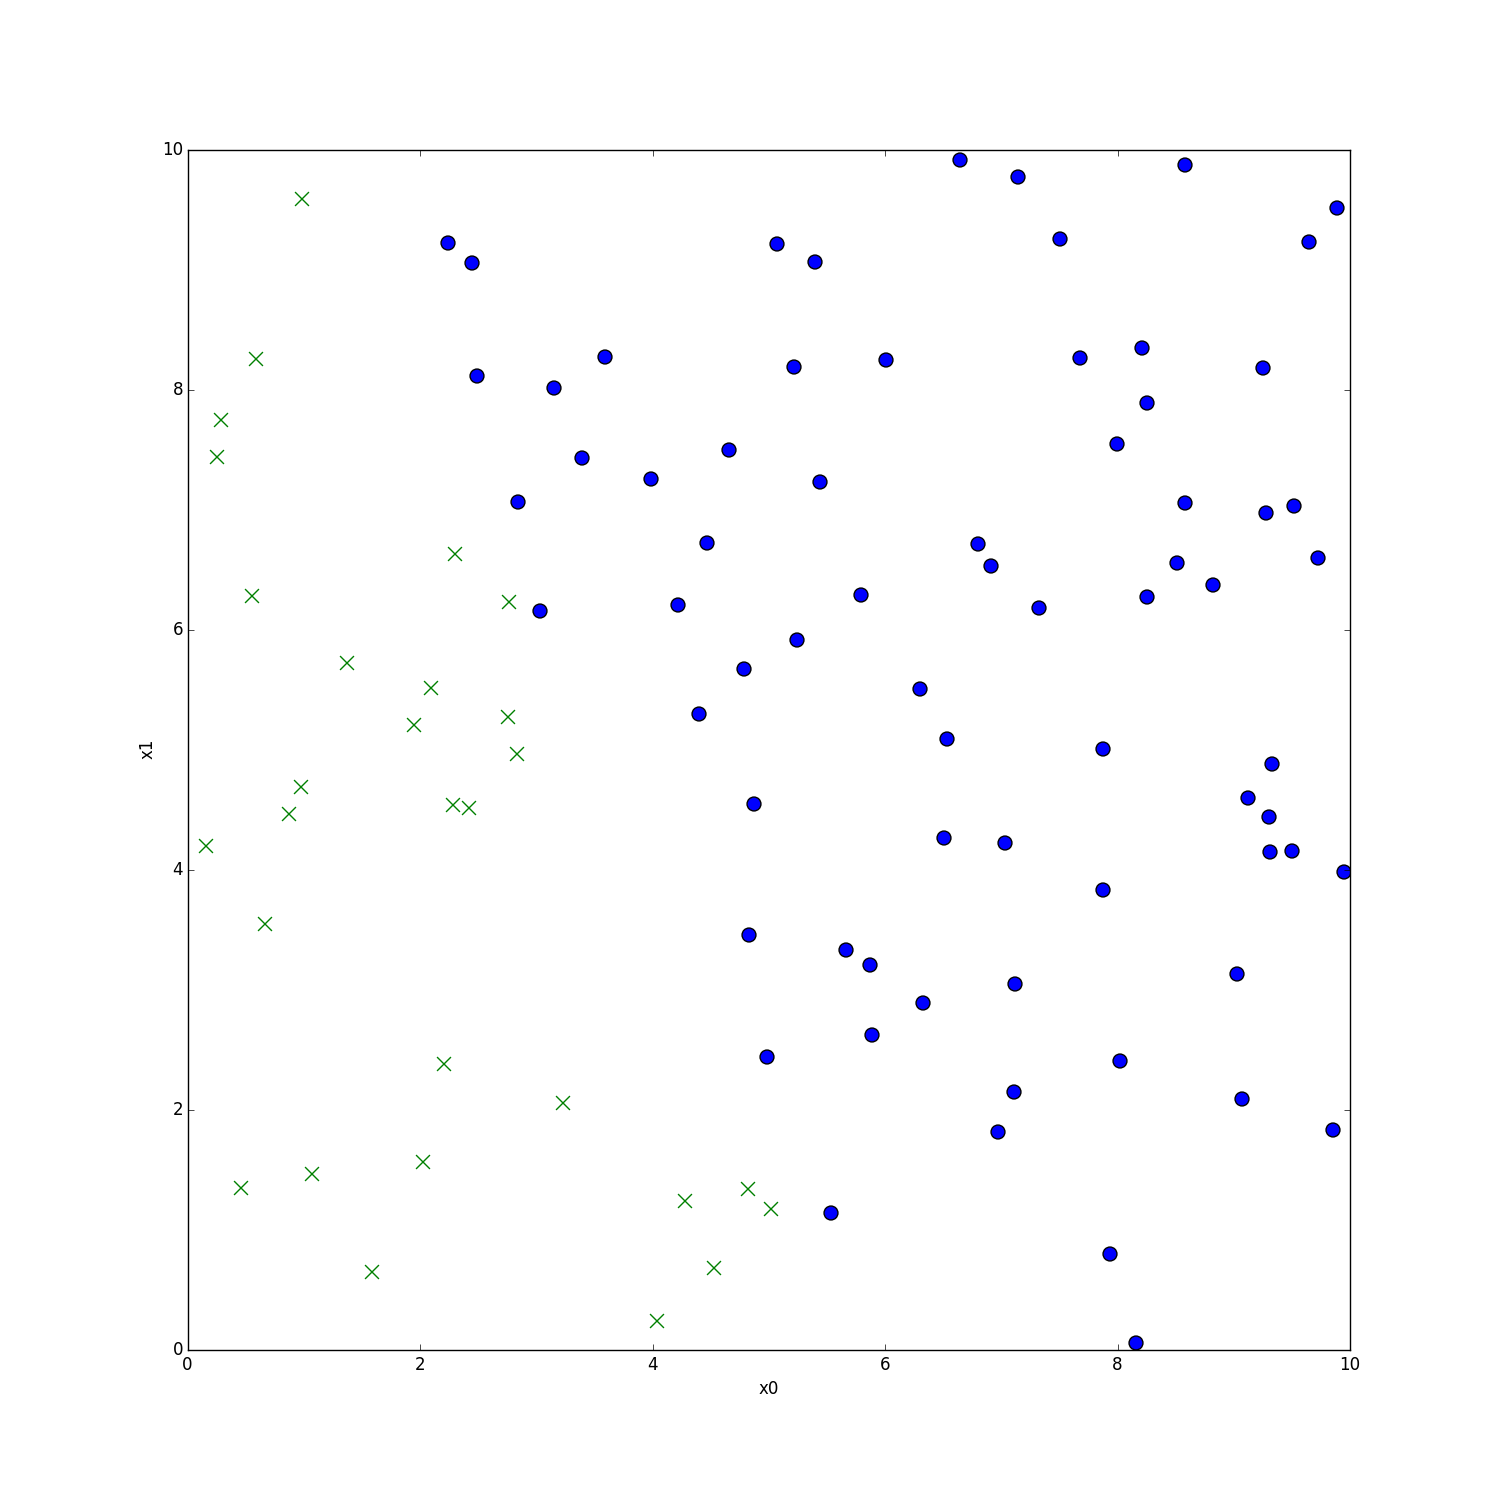
\includegraphics[scale=0.2]{./pictures/logreg_db000.png}
  \end{center}
\end{frame}

\begin{frame}
  \begin{center}
    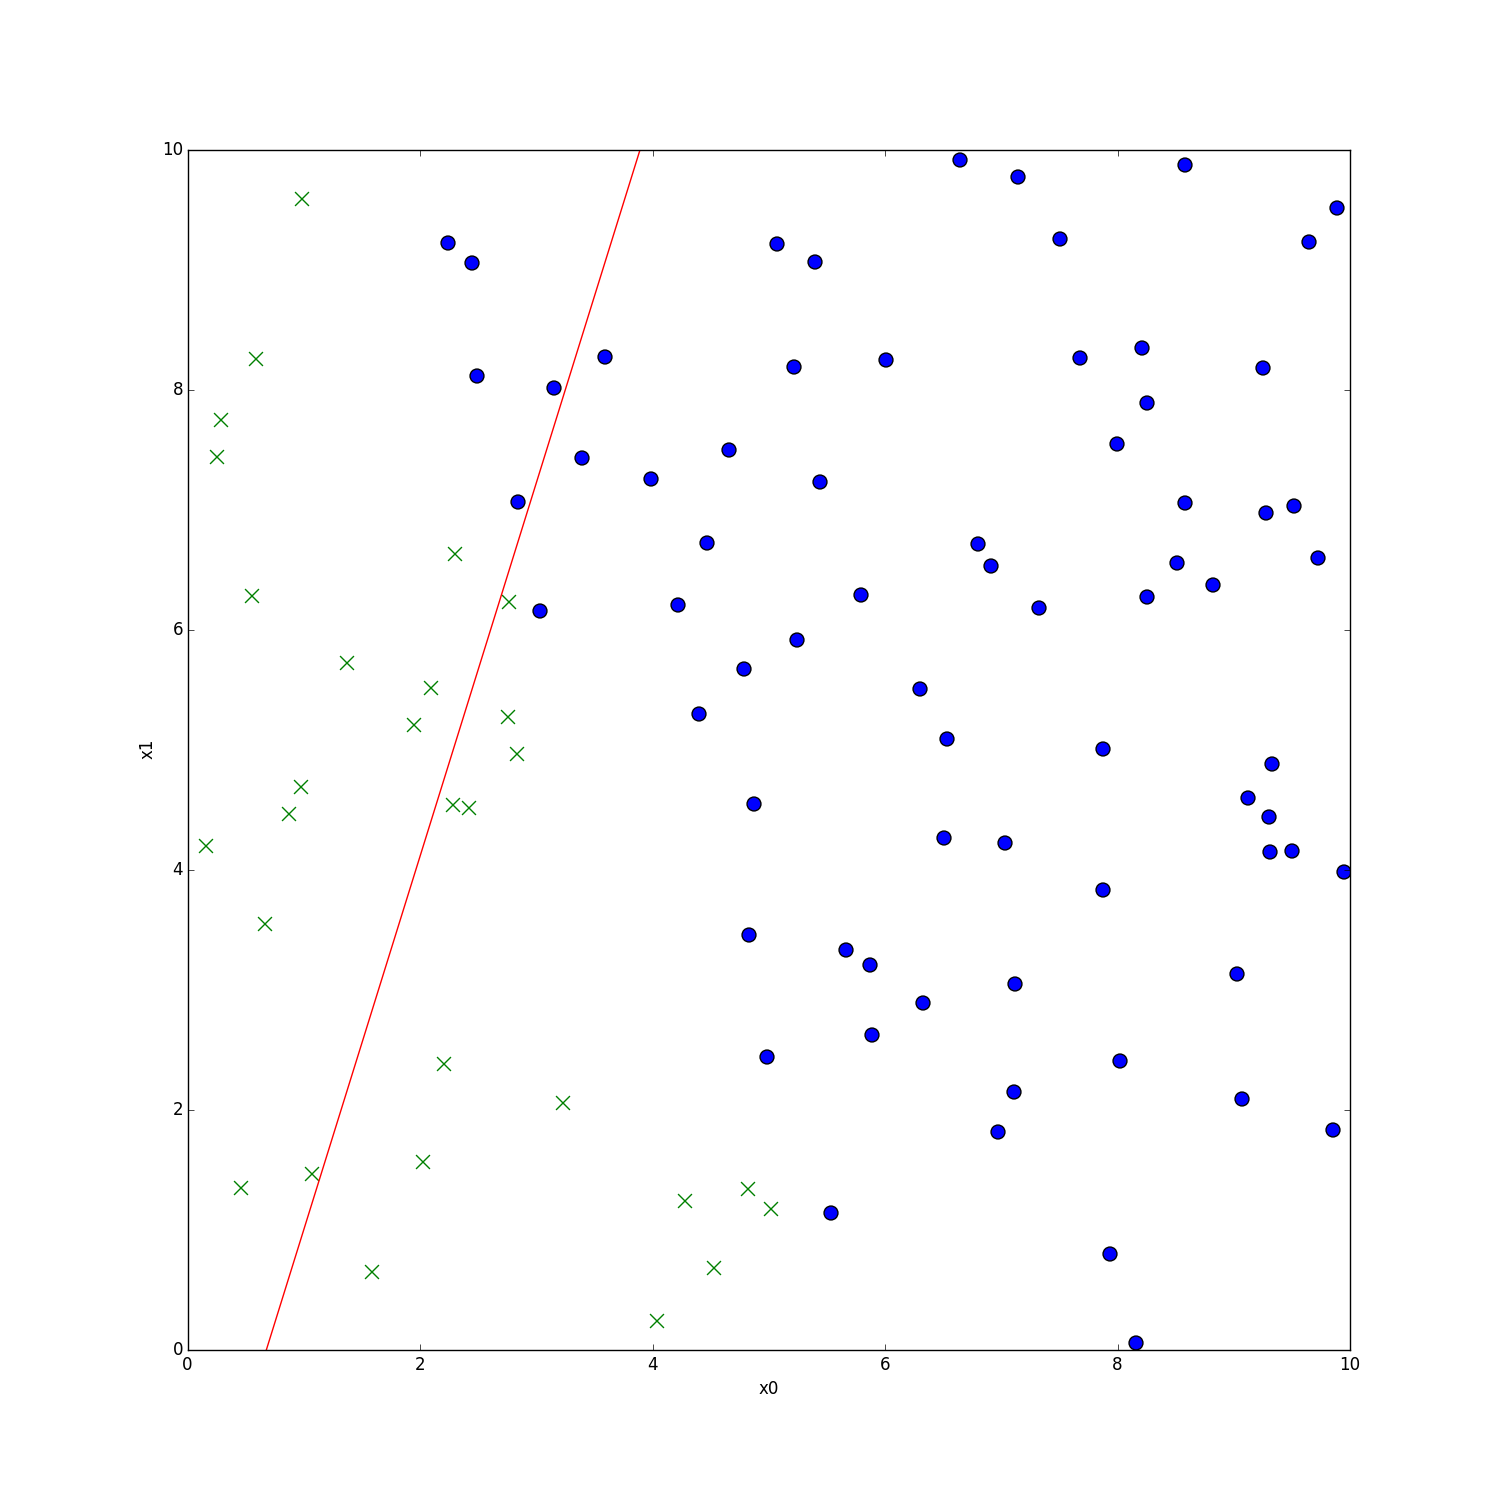
\includegraphics[scale=0.2]{./pictures/logreg_db001.png}
  \end{center}
\end{frame}

\begin{frame}
  \begin{center}
    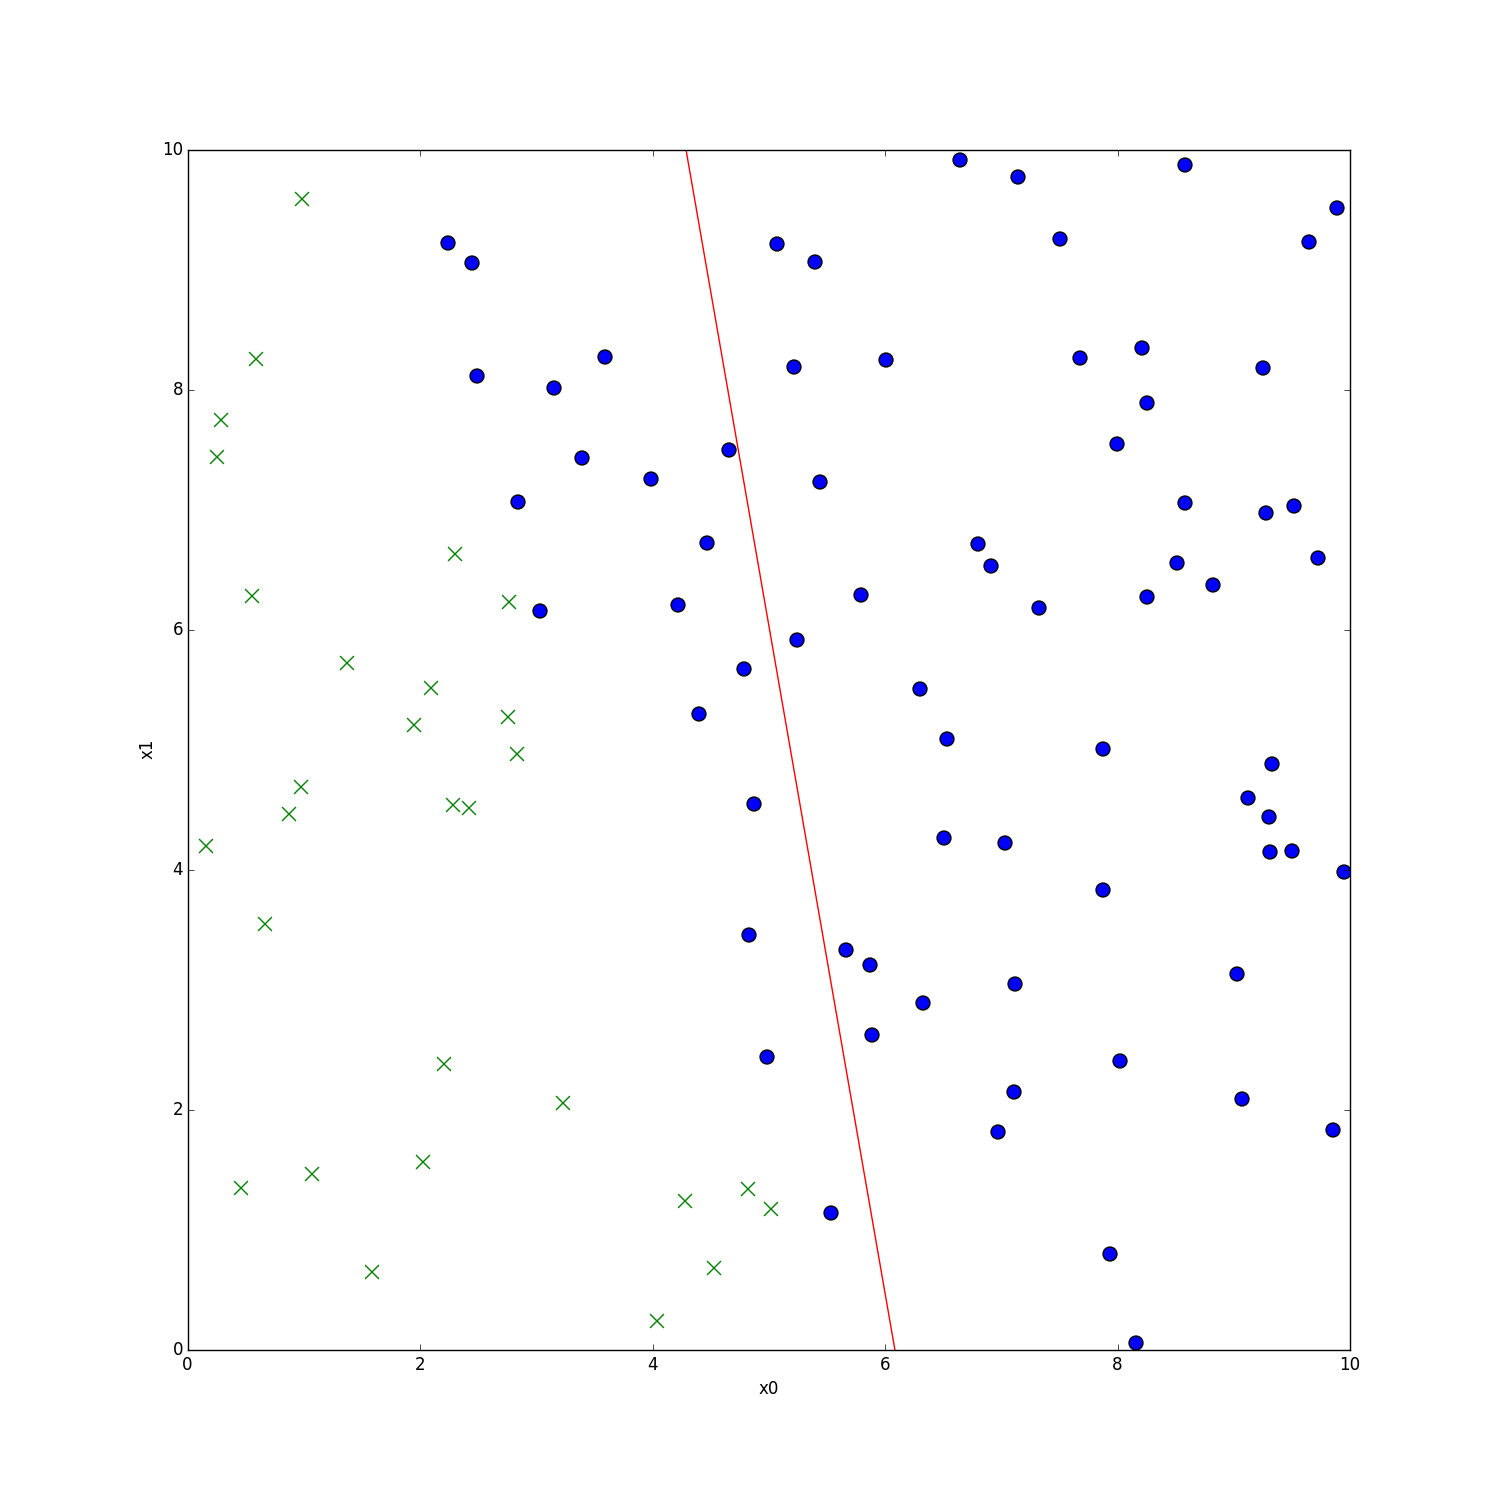
\includegraphics[scale=0.2]{./pictures/logreg_db012.png}
  \end{center}
\end{frame}

\begin{frame}
  \begin{center}
    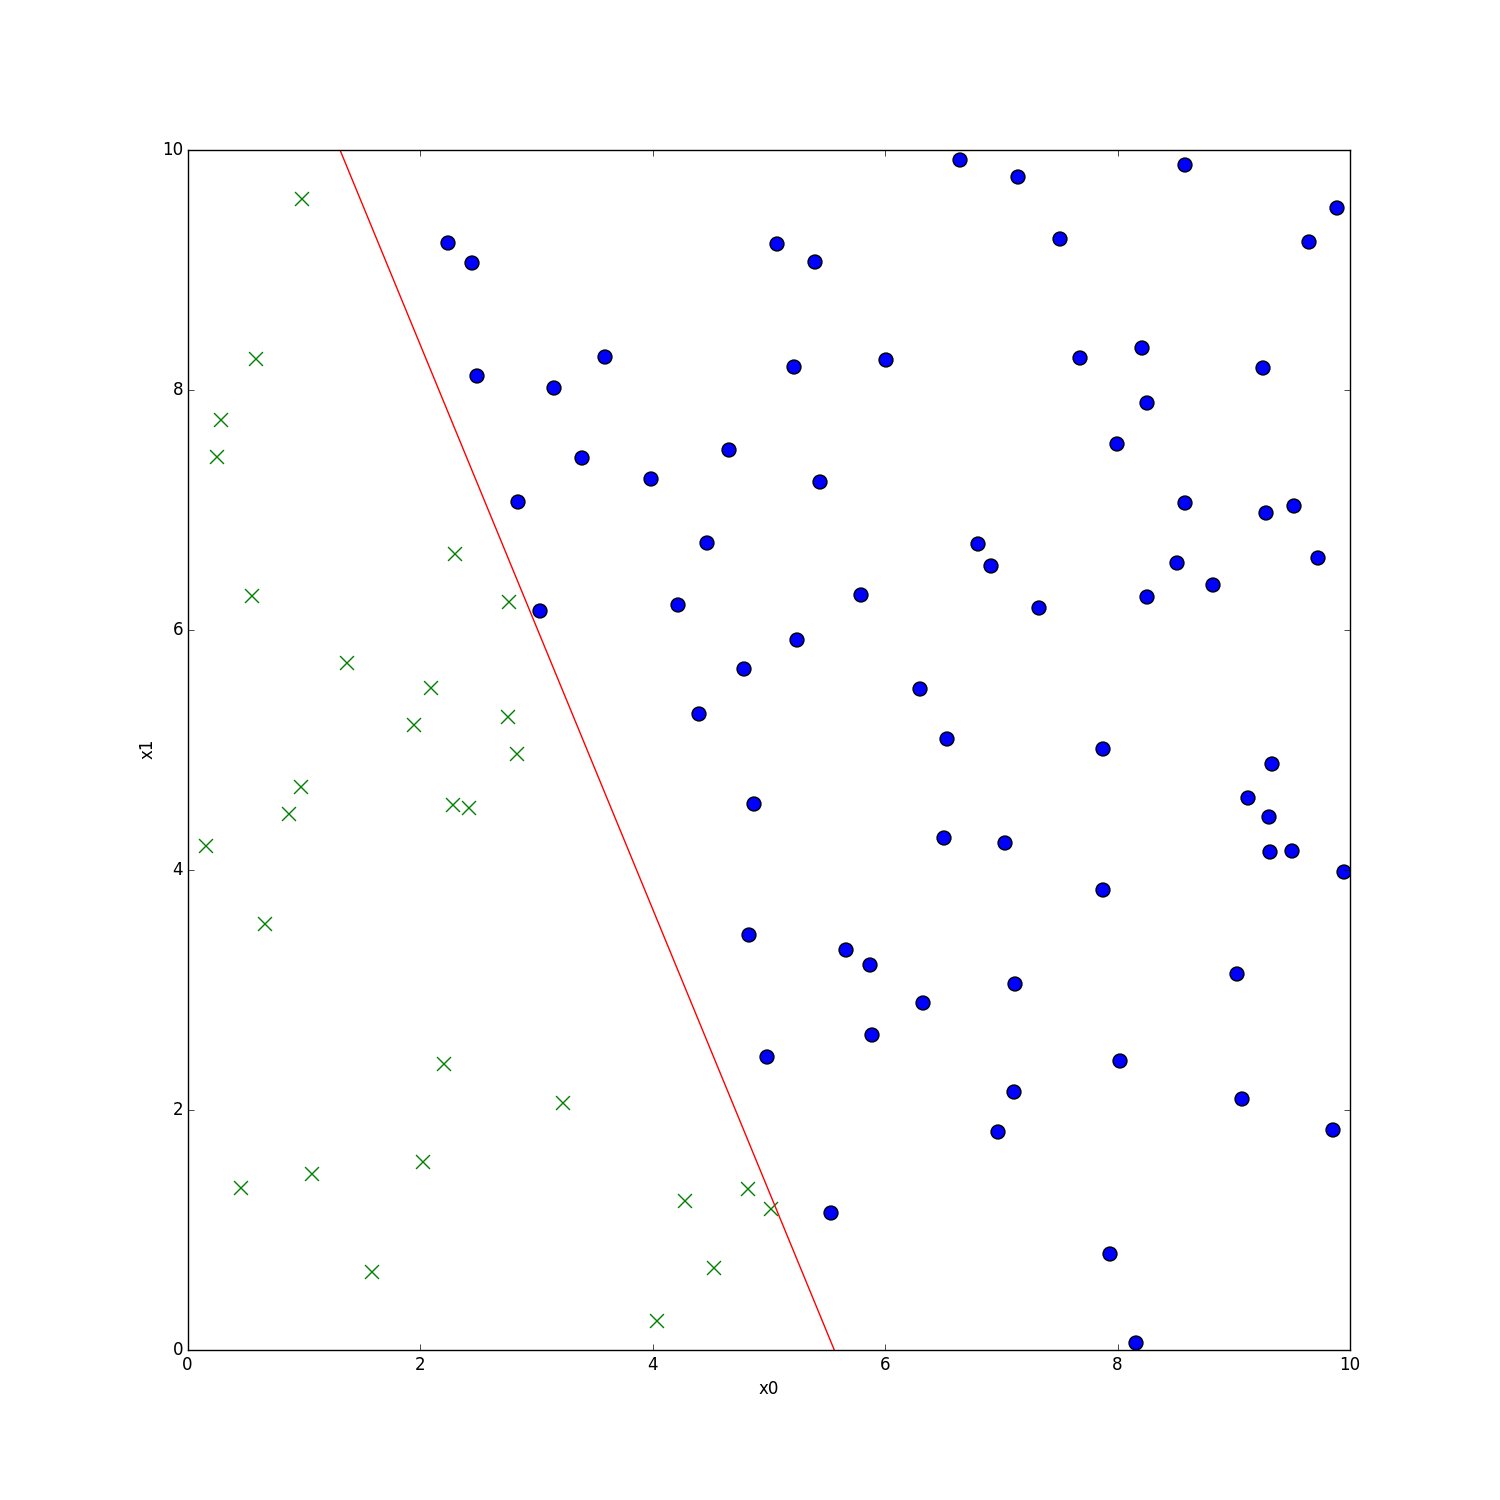
\includegraphics[scale=0.2]{./pictures/logreg_db078.png}
  \end{center}
\end{frame}

\begin{frame}
\begin{center}
  $
  \begin{array}{cc}
      &
      \left(
        \begin{matrix}
          \only<2>{w_0 \\}
          w_1 \\
          \vdots \\
          w_n
        \end{matrix}
      \right) \\
    &\\
    \left(
      \begin{matrix}
        \only<2>{1 &} x_1 & \ldots & x_{n}
      \end{matrix}
    \right) & {\left(\textbf{x} \cdot \textbf{w} \right)}
  \end{array}
  \hspace{2em}
  $
\only<1>{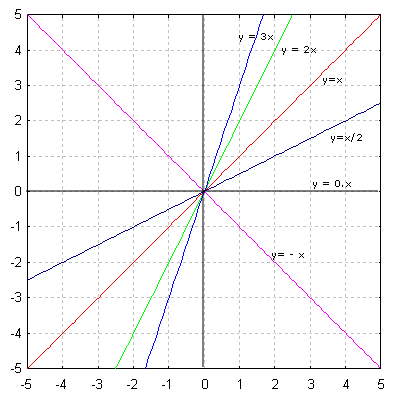
\includegraphics[scale=0.3]{./pictures/linear.png}}
\only<2>{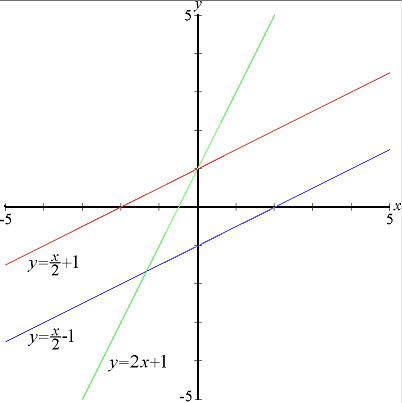
\includegraphics[scale=0.3]{./pictures/affine.png}}
\end{center}
\end{frame}
